\section{Schéma simplifié du cycle de vie d'un projet}
\newImageAnnexe[H]{0.75}{cycle-vie-projet.png}{cycleVieProjet}

\clearpage
\section{Construction des modules communs de l'application au sein d'un projet \naq}

\normalsize{GOP = Groupe onepoint}

\newImageAnnexe{0.9}{modules.png}{commons-modules}

\clearpage
\section{Build continu d'un projet \naq}
\begin{figure}[ht]
	\centering
	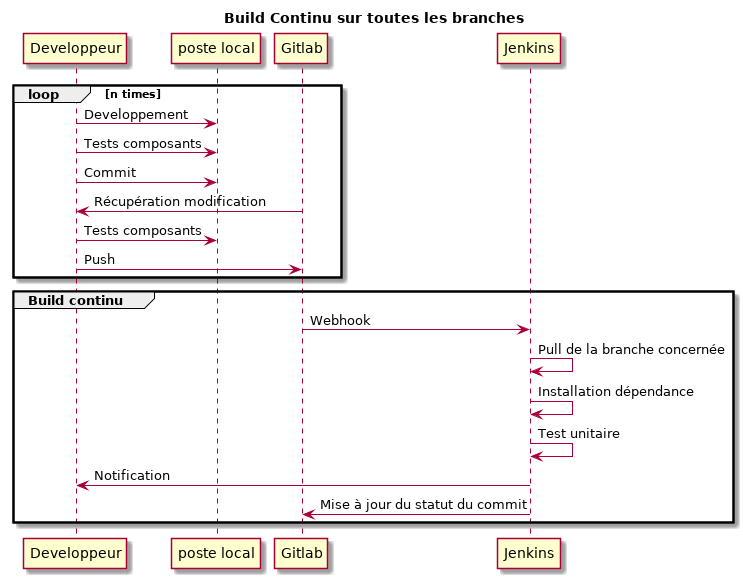
\includegraphics[scale=0.6,angle=-90]{img/build-continu.png}
	\label{annexe:build-continu}
\end{figure}

\clearpage
\section{Flux de travail du déploiement d'une version d'un site \naq}
\newImageAnnexe{0.32}{release.png}{release-naq}

\clearpage
\section{Matrice de développement \devops}

Source : \url{https://www.infoq.com}

Dans l'image ci-dessous, on peut distinguer une matrice permettant à une entreprise de situer son niveau dans l'adoption d'une démarche \devops. Cette matrice est constituée de 5 niveaux, chacun demandant plus ou moins d'effort pour être atteint et permet de juger 5 points clés, le premier étant la culture de l'entreprise et la façon dont elle est organisée. Cela correspond à la façon l'entreprise va prioriser le travail et organiser les décisions à prendre.

Le second point concerne l'architecture des systèmes que l'entreprise crée. Plus l'entreprise est mature sur ce sujet, plus elle pourra centraliser et versionner chaque changement d'infrastructure, sans avoir à intervenir manuellement sur le projet pour des changements de structure de base de données par exemple. 

Le troisième point concerne la façon dont sont déployées les applications, l'objectif ultime étant de n'avoir aucune intervention humaine sur toute la chaine de déploiement. Le quatrième test concerne la vérification des critères d'acceptations et la qualité des tests mis en place sur le projet. Le dernier point concerne quant à lui la façon dont sont gérés les informations et logs de l'application ainsi que la façon dont ils sont exploités.

\begin{figure}[ht]
	\centering
	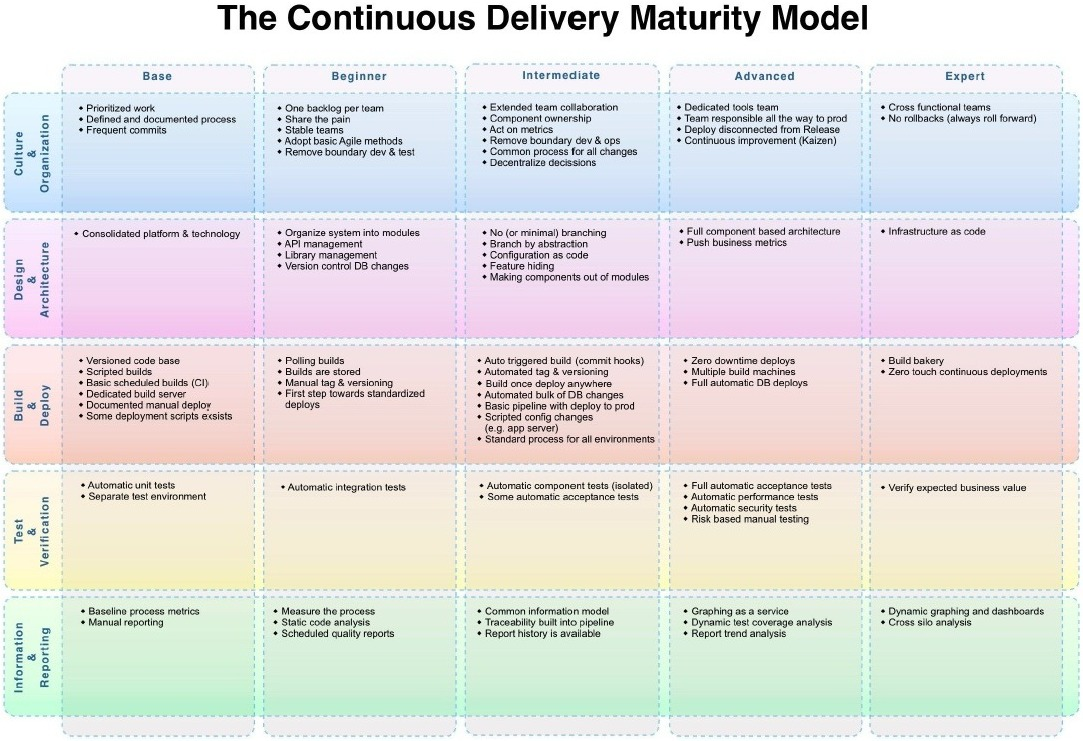
\includegraphics[scale=0.62,angle=-90]{img/devops-matrice.jpg}
	\label{annexe:devops-matrice}
\end{figure}

\clearpage
\section{Exemple d'erreurs détectées par PHPStan}

Dans l'exemple ci-dessous, PHPStan retournera une erreur indiquant que le paramètre requis \frquote{\$type} n'a pas été renseigné, ainsi qu'une erreur indiquant que la méthode privée \frquote{internalBehaviour} ne peut être utilisée en dehors de la classe. 

Il est à noter que cette analyse statique de code peut être et est souvent effectuée au sein de l'\gls{IDE} pour permettre une détection de l'erreur au plus tôt.

%%TC:ignore
\begin{minted}[linenos]{php}
<?php
// index.php

require_once(__DIR__."/vendor/autoload.php");
$a = new \App\File();
$content = $a->loadFile("file.json");
$a->internalBehaviour();

// src/File.php

namespace App;

class File {
  public function loadFile($file, $type) {
    $content = file_get_contents($file);
    if ($type == "json") {
      return json_decode($file);
    }
    return $content;
  }
  
  private function internalBehaviour() {
    echo "this is not public";
  }
}

// ------ ------------------------------------------------------------------- 
// Line   index.php                                                          
// ------ ------------------------------------------------------------------- 
// 6      Method App\File::loadFile() invoked with 1 parameter, 2 required.  
// 7      Call to private method internalBehaviour() of class App\File.      
// ------ ------------------------------------------------------------------- 

\end{minted}
\label{annexe:php-error}
%%TC:endignore
